\documentclass[a4paper]{article}[11pt]
\usepackage[left=3cm, right=3cm, top=3cm, bottom=2cm,marginparwidth=1.75cm]{geometry}
\usepackage[utf8]{inputenc}
\usepackage{indentfirst}
\usepackage{amsmath}
\usepackage{textgreek}
\usepackage{fixltx2e}
\usepackage{listings}
\usepackage{color}
\usepackage{graphicx}
\graphicspath{ {images/} }
\usepackage{subcaption}

\definecolor{green}{rgb}{0,0.6,0}
\definecolor{gray}{rgb}{0.5,0.5,0.5}
\definecolor{mauve}{rgb}{0.58,0,0.82}

\lstset{ %
  backgroundcolor=\color{white},   
  basicstyle=\footnotesize,       
  breaklines=true,                 
  captionpos=b,                    
  commentstyle=\color{green},    
  escapeinside={\%*}{*)},          
  keywordstyle=\color{blue},       
  stringstyle=\color{mauve}, 
}



\title{Influence of mixture composition and initial pressure on the autoignition temperature of methane-air mixture}
\date{26.04.2017}
\author{\\
\\
Cezary Kardaś}

\begin{document}
	\maketitle
    \pagenumbering{gobble}
    \newpage    
  

	\newpage
    \pagenumbering{arabic}
    
    \section{Abstract}
    	
	Methane  CH\textsubscript{4} is an easily combustible gas that is produced on a global scale by natural sources such as wetlands and the oceans. However, human sources account for as much as 64\%  of total global emissions. Methane is widely used in numerous industrial processes as a reagent or a fuel source. It is also an important byproduct of livestock farming, for massive amounts of methane are exhaled daily by the livestock due to fermentation taking place during digestion of plant matter in their stomachs.\par 
    At the same time, methane is also heavily contributing to the green house effect which is major concern for mankind. For that reason actions have been taken to first and foremost limit global methane emissions and secondly use the gas appropriately instead of releasing it directly into the atmosphere. Such actions require a safe and secure way to store the gas seeing how it is often produced in close proximity of inhabited areas. An improper method of gaseous methane storage could be a direct cause of an autoignition and therefore of a violent explosion which could easily damage property or injure individuals. \par 
    The aim of this study is to determine how boundary conditions such as initial pressure and equivalence ratio of methane influence the autoignition temperature of a methane-air mixture which usually fills the storage containers. The results could potentially lead to development of guidelines for safe methane-air mixture storage.   \par 
    
      
    \section{Auto-ignition theory}
    The autoignition temperature (AIT) of a gaseous mixture of fuel and oxidizer is the lowest possible temperature at which the mixture ignites spontaneously i.e. without an outside source of ignition such as an electrical spark or an open flame. The enthalpy of the mixture at autoignition temperature is high enough to serve as a source of activation energy for the process of combustion. \par
    
    In the case of methane, which is the shortest hydrocarbon in terms of average carbon chain length, this activation energy is the highest of all hydrocarbons. Longer and therefore heavier (per unit volume) hydrocarbons tend to auto-ignite before methane does.  \par
\begin{figure}[h]
\centering
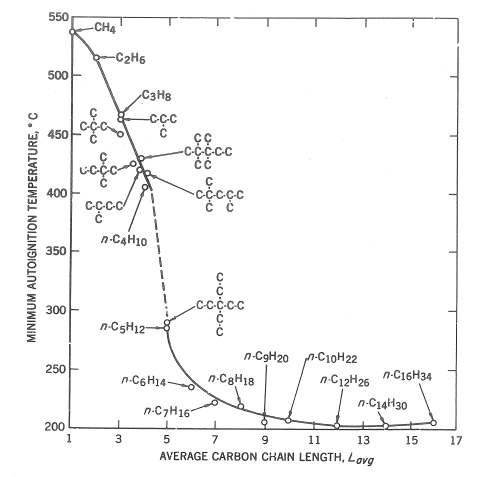
\includegraphics[width=5cm]{zabetakis.PNG}
\caption{AIT as a function of carbon chain length (Zabetakis\textsuperscript{[4]})}
\end{figure}
    Said combustion process is a chain of hundreds of different chemical reactions. The initial reactions heat up the mixture through slow oxidation which incites faster reactions which cause the actual autoignition. The chain could be described with one global equation: \par
    
    \begin{equation*}
    	CH_4 + O_2 = CO_2 + 2 H_2O\\        
    \end{equation*}
    or in case of combustion in air:
    \begin{equation*}
    	CH_4 + 2*(O_2+3.76N_2) = CO_2 + 2*H_2O + 7.52 N_2 
     \end{equation*}
     
     As shown in the equation, in case of methane-air combustion, for every mole of methane 9.52 moles of air are necessary for stoichiometric combustion. The ratio of the mixture's fuel-to-oxidizer ratio to stoichiometric fuel-to-oxidizer ratio is called an equivalence ratio of said mixture - \textphi . \par 
     
     \begin{gather*}
    FAR = \frac{n_{fuel}}{n_{air}} \\
    n = number \ of \ moles \\
    \phi = \frac{FAR}{FAR_{stoichiometry}}
     \end{gather*}
     
      \textphi \ greater than one means that the mixture is rich and not all of the the fuel undergoes combustion due to lack of oxidizer. Alternatively, \textphi \ lower than one indicates a lean mixture which has an excess of oxidizer. \par 
      Another way to describe the composition of a mixture is to use molar fractions. Molar fraction is the ratio of the number of moles of any given component to the overall number of moles of a mixture. \par 
      
      \begin{gather*}
    X_{fuel} = n_{fuel}/n_{mixture}
     \end{gather*}
     
     Determining the auto-ignition temperature through analysis of the chain reaction alone is impossible. Therefore using experimental methods and simulations are necessary.
     
    \section{Simulation}
    
    \subsection{Methodology}
    	The analysis of the autoignition temperature as a function of the initial parameters of the mixture is based on the results of a simulation utilizing Cantera suite for chemical kinetics calculations in Python. The simulation is run inside a reactor network comprising a singular 0-dimensional adiabatic reactor. \par 
        A perfectly homogeneous methane-air mixture is placed inside at t=0 and its parameters i.e. molar fractions of its components, initial temperature and initial pressure are set. Subsequently, simulation time advances by 600s which according to previous studies is in most cases a long enough period for auto-ignition to occur even with long periods of slow oxidation. Only one time step was used in order to minimize computing time since autoignition delay time is irrelevant to this study. \par 
        Autoignition is determined to have had occurred if the temperature inside of the reactor is at least 200K higher than initially. Every set of parameters resulting in an autoignition is stored for later use in graphs. \par
        The simulation first finds the autoignition temperature of a 60\% methane-air mixture as a function of pressure between 0,05 MPa and 3,5 MPa by finding the AIT every 50 kPa. This part of the study is designated as Task 1. \par
        Task 2 of the program is finding how the AIT changes with the equivalence ratio. Here, a set pressure of one atmosphere was used while the number of moles of methane changed from 0.2 to 8 with a step of 0.3 moles. It was then subsequently converted into equivalence ratios.  \par 
        For the sake of calculation speed, the autoignition temperature is first approximated within a 50-Kelvin-wide window. Then, more precise calculations take place within that window in order to determine the AIT down to one Kelvin. In task 1, the desired precision is 0.5K. In task 2 1K is sufficient.
    
    \subsection{Code description}
\begin{lstlisting}[language=Python]
#importing necessary libraries
import numpy as np 
from cantera import *
import matplotlib.pyplot as plt
from scipy.optimize import curve_fit

#selecting reaction mechanisms
gas = Solution('gri30.xml')

#setting minimal, maximal temperature and two step sizes
Tmin=500
Tmax=1500
temp_step=0.5
temp_step_coarse=50

#setting minimal, maximal pressure and a step size
Pmin=100000
Pmax=3500000
P_step=50000

#setting time step size
time_step=600



#calculating number of temperature loop iterations for different levels of precision
temp_steps_coarse_no=int(((Tmax-Tmin) // temp_step_coarse)+1)
temp_steps_no=int((temp_step_coarse// temp_step)+1)

#calculating number of pressure loop iterations
P_steps_no=((Pmax-Pmin)//P_step)+1

#creating storage arrays
autoign_temp = []
autoign_P=[]
autoign_temp_X=[]
autoign_X=[]
autoign_X_fr=[]
autoign_X_FAR=[]

#initializing stoichiometric fuel-to-air ratio
FARst=0.5/4.76

#TASK1 - AIT as a function of initial pressure
print ("Task 1")
#setting initial pressure for the pressure loop
P=Pmin

#pressure loop start
for p in range (0, P_steps_no):  
    
    #setting default state of trigger variable
    auto=0 
    
    
    #setting initial temperature for the approximate temperature loop
    T=Tmin
    
    #approximate temperature loop start
    for tc in range(0,temp_steps_coarse_no):
        #creating the gas, the reactor and the reactor network
        #for 4.76 moles of air, 7.14 moles of methane translate to 60% molar fraction
        gas.TPX = T, P, 'CH4:7.14,O2:1,N2:3.76'
        r=IdealGasReactor(gas)
        net=ReactorNet([r])
        
        #advancing simulation time 
        net.advance(time_step)
         
        #checking whether autoignition occured   
        if (r.T-T)>200:
            #setting the mixture's temperature to the lower limit of the approximate temperature window
            T-=temp_step_coarse
            
            #precise temperature loop start 
            for t in range(0,temp_steps_no):
                #creating the gas, the reactor and the reactor network for precise calculations
                #temperature and pressure change with iterations, mixture composition is constant
                gas.TPX = T, P, 'CH4:7.14,O2:1,N2:3.76'
                r=IdealGasReactor(gas)
                net=ReactorNet([r])
                
                #advancing simulation time 
                net.advance(time_step)
                
                #checking whether autoignition occured 
                if (r.T-T)>200:
                    #setting trigger variable value to break the outer loop 
                    auto=1
                    #storing current initial temperature and pressure in arrays
                    autoign_temp.append(T)
                    autoign_P.append(P/1000000)
                    #printing current initial conditions
                    print ("X: 7.14, T: ",'%.1f' % T, "P: ", P)
                    #breaking the precise temperature loop, AI occured
                    #higher temperatures do not need to be verified
                    break
                #raising the initial precise temperature in case autoiginition didn't occur    
                T+=temp_step 
                
        #breaking the approximate temperature loop if AI occured
        #higher temperatures do not need to be verified
        if auto==1:
            break    
        #raising the initial approximate temperature in  case autoiginition didn't occur    
        T+=temp_step_coarse
    #raising the pressure   
    P+=P_step


#storing results as x, y for clarity
x = autoign_temp
y = autoign_P
 
#setting plot size
plt.figure(figsize=(7,5))

#creating,labeling and saving the Initial Pressure vs AIT plot
plt.plot(x, y, '-', color='orange') 
plt.grid()
plt.xlabel("Autoignition Temperature [K]")
plt.ylabel(r'Initial Pressure [MPa]')
plt.savefig('1.png', bbox_inches='tight')
plt.show()


#TASK2 - AIT as a function of equivalence ratio
print ("-----------------")
print ("Task 2")
#setting minimal, maximal number of moles of methane, step size
X_min=0.2
X_max=8
X_step=0.3

#calculating number of molar loop iterations
X_steps_no=int((X_max-X_min)//X_step+1)


#setting initial number of moles
X=X_min

#changing the precision of calculations - raising the size of temperature step
#calculating new number of steps
temp_step=1
temp_steps_no=int((temp_step_coarse// temp_step)+1)

#molar loop start
for x in range(0, X_steps_no):
    #setting default state of trigger variable
    auto = 0
    #setting initial temperature for the approximate temperature loop
    T=Tmin
    #approximate temperature loop start
    for tc in range(0,temp_steps_coarse_no):
        #creating the gas, the reactor and the reactor network for approximate calculations
        #temperature mixture composition change with iterations, pressure is constant and equal to one atmosphere
        #calculations look just like in Task 1 
        gas.TPX = T, one_atm, {'CH4':X,'O2':1,'N2':3.76}
        r=IdealGasReactor(gas)
        net=ReactorNet([r])
       
        net.advance(time_step)
        
        if (r.T-T)>200:
            
            T-=temp_step_coarse
           
            for t in range(0,temp_steps_no):
                gas.TPX = T, one_atm, {'CH4':X,'O2':1,'N2':3.76}
                r=IdealGasReactor(gas)
                net=ReactorNet([r])
                net.advance(time_step)
                if (r.T-T)>200:
                    auto=1
                    autoign_temp_X.append(T)
                    autoign_X.append(X/(X+4.76))
                    autoign_X_FAR.append((X/4.76)/FARst)
                    print ("X: ", '%.1f' % X , "T: ", T, "P: ", '%.0f' % one_atm)
                    break
                T+=temp_step 
        if auto==1:
            break
                
        T+=temp_step_coarse
    X+=X_step
    
#creating plots
y2 = autoign_temp_X
x2 = autoign_X


plt.figure(figsize=(7,5))
plt.plot(x2, y2, '-', color='orange')
plt.grid()
plt.xlabel(r'Molar fraction of methane')
plt.ylabel("Autoignition temperature [K]")
plt.savefig('2.png', bbox_inches='tight')
plt.show()


y3 = autoign_temp_X
x3 = autoign_X_FAR

plt.figure(figsize=(7,5))
plt.plot(x3, y3, '-', color='orange')
plt.grid()
plt.xlabel(r'Equivalence ratio')
plt.ylabel("Autoignition temperature [K]")
plt.savefig('3.png', bbox_inches='tight')
plt.show()


        	
\end{lstlisting}
    \newpage
    \section{Results}
    \subsection{Task 1 - initial pressure vs AIT}
\begin{figure}[h]
\centering
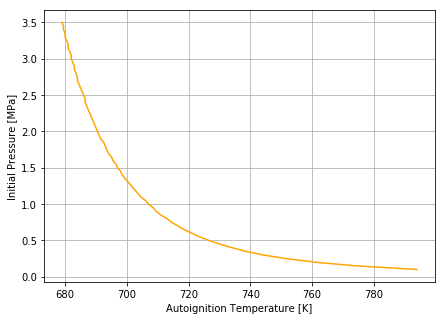
\includegraphics[width=8cm]{1.png}
\caption{Results of Task 1. Minimal initial temperature for which autoignition occurs as a function of initial pressure}
\end{figure}

Task 1 resulted in a direct exponential correlation between initial pressure and autoiginiton temperature (Figure 1). The higher the initial pressure, the lower the AIT since pressure contributes a bigger part of the mixture's enthalpy. These findings correspond to the results of Frederik Norman's study\textsuperscript{[1]} presented in the Fig. 3. 

\begin{figure}[h]
\centering
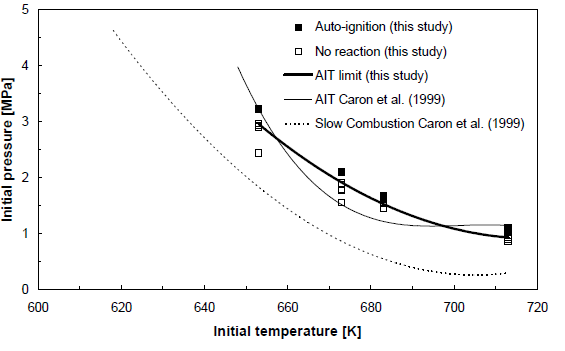
\includegraphics[width=8cm]{norman.PNG}
\caption{Results of Norman's study. Initial pressure vs AIT}
\end{figure}

The study determined that the autoignition temperature of 60\% methane-air mixture in atmospheric conditions is roughly 707K. 


\newpage
\subsection{Task 2 - mixture composition vs AIT}
\begin{figure}[h]
\begin{subfigure}{.5\textwidth}
\centering
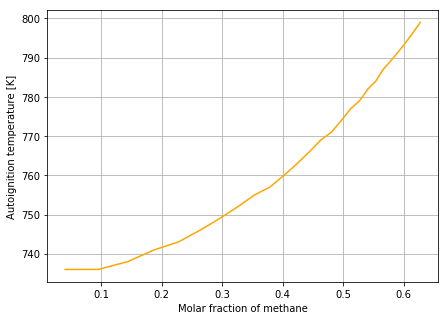
\includegraphics[width=8cm]{2.png}
\caption{AIT as a function of molar fraction of methane}
\end{subfigure}
\begin{subfigure}{.5\textwidth}
\centering
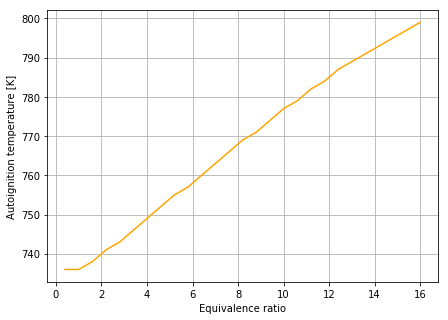
\includegraphics[width=8cm]{3.png}
\caption{AIT as a function of equivalence ratio}
\end{subfigure}
\caption{Results of Task 2}
\end{figure}

Results of Task 2 show near linear correlation between mixture's equivalence ratio and its autoignition temperature. Starting at \textphi = 1 raising the equivalence ratio by 1 raises the AIT by 9K. Little to no change in AIT was found for lean mixtures. The AIT of a stoichiometric mixture (\textphi = 1) is 

    \section{Conclusions}
    The aim of the study was to determine the influence of pressure and mixture composition on the autoignition temperature of gaseous methane in air in order to find its safe storage conditions. The study found that lowering storage pressure is favorable. At pressures close to atmospheric pressure, lowering the pressure by 100kPa raises the AIT by around 20K. Furthermore, it is safer to store rich mixtures due to them having higher AIT than lean mixtures.
    
    \section{References}
    
\begin{enumerate}
\item  Frederik Norman, \textit{Influence of Process Conditions On The Auto-Ignition Temperature of Gas Mixtures}, Katkolieke Universiteit Leuven, Faculteit Ingenieurswetenschappen, June 2008
\item SAFEKINEX, \textit{Report on experimentally determined self-ignition temperature and the ignition delay time, Federal Institute for Materials Research and Testing}, 2002 
\item Anne Felden, \textit{CANTERA Tutorials}, Tutorial 4, CERFACS, November 2015 
\item Zabetakis, M.G., Rurno, A.L. and Jones, \textit{Minimum spontaneous
ignition temperatures of combustibles in air}, Industrial Engineering Chemistry, 1954
2173–2178
\end{enumerate}
    
\end{document}
